\documentclass[11pt]{article}
\usepackage{amsmath}
\usepackage{amsfonts}
\usepackage{graphicx}
\usepackage{hyperref}
\usepackage{url}
\usepackage{xcolor}
\usepackage{xspace}
\usepackage{microtype}
\usepackage{booktabs}
\usepackage{fancyhdr}
\usepackage{lipsum}
\usepackage{siunitx}
%%%% added
\usepackage[backend=biber, doi = false, sorting=none]{biblatex}
\addbibresource{bibliography.bib}
\usepackage{biblatex2bibitem}
% \usepackage{cite}
\usepackage{csquotes}
\usepackage{tabularx}
\usepackage{makecell}
%%%%%%%%
\usepackage[utf8]{inputenc} % allow utf-8 input
\usepackage[T1]{fontenc}
\usepackage[a4paper, left=2.1cm, right=2.1cm]{geometry}
% Load the parskip package with skip and indent options
\usepackage[skip=8pt plus1pt, indent=20pt]{parskip}
\setlength{\headheight}{14pt}
\addtolength{\topmargin}{-2pt}
\pagestyle{fancy}
\rhead{}
\fancyhead[LO]{Covid remittances}
% Custom math commands
\newcommand{\E}{\operatorname{e}}
\newcommand{\defin}{\coloneqq}
\newcommand{\D}{\mathop{}\!\mathrm{d}}
\newcommand{\Dt}[1][t]{\D#1}
\newcommand{\incar}{\mathcal{I}}
\newcommand{\transv}{\tau}
\renewcommand{\familydefault}{\sfdefault}

\renewcommand{\appendixname}{Supplementary Material}

\usepackage{lmodern}
\usepackage{amssymb}
\usepackage{enumitem}
\newcommand{\expit}{\operatorname{expit}}

% Draft of 3 Nov 2026, written from 2026-10-30/ (model plan, calibration, shock runs, household layer).
% Figure paths are relative to 2026-10-30/. New references: see paper_draft_new_refs.bib.
% Shock-year numbers come from the quick map (kappa 0, 0.5, 0.8, 1; beta fitted per kappa); the full map
% is still to be run and may move them slightly.

\title{Families stepped in: why remittances to Mexico held up during COVID-19}

\author{\href{https://orcid.org/0000-0002-3899-1175}{\includegraphics[scale=0.06]{orcid.pdf}\hspace{1mm}Andrea Vismara*} \\
    Complexity Science Hub\\
    Metternichgasse 8\\
    1030 Vienna, Austria \\
    \texttt{vismara@csh.ac.at} \\
    \and
    \href{https://orcid.org/0000-0002-0738-2633}{\includegraphics[scale=0.06]{orcid.pdf}\hspace{1mm}Rafael Prieto-Curiel} \\
    Complexity Science Hub\\
    Metternichgasse 8\\
    1030 Vienna, Austria \\
    \texttt{prieto-curiel@csh.ac.at} \\
}

\hypersetup{
pdftitle={Families stepped in: why remittances to Mexico held up during COVID-19},
pdfauthor={Andrea~Vismara, and Rafael~Prieto-Curiel},
pdfkeywords={Human migration, International remittances},
}


\begin{document}
\maketitle

\begin{abstract}
{
When COVID-19 hit, forecasters expected remittances to collapse as migrants lost their jobs. Remittances to Mexico did not fall: transfers held up in 2020 and rose well above trend in 2021 and 2022. We build a model on the real family networks of 3,405 Mexican households and their 7,999 relatives in the United States, calibrate how often migrants want to send in normal times, and then expose the networks to the job losses of the pandemic and to the death toll in Mexico. Job losses alone would have cut transfers by 12\% in spring 2020; the data show 3\%. The gap closes only if relatives replaced almost every migrant who lost their job, and two independent features of the data, the depth of the spring 2020 drop and the size of the jumps when US stimulus checks arrived, both point to one-for-one replacement. The rise of 2021 is matched by a modest, lasting response to the cumulative toll of the crisis in Mexico, and the same response predicts 2022, a year the model was not fitted to. Behind the national stability, losses were concentrated: households linked to a single migrant could not be helped, and half of all lost months of income fell on fewer than one household in a hundred.
}
\end{abstract}

\vspace{1em}
\noindent \textbf{Keywords:} Human migration, International remittances
\vfill
* Corresponding author

%% main corpus
\newpage
\section{Introduction}

\subsection{what is the problem? why is it relevant?}
{
Remittances are the money migrants send to their families at home \cite{ratha2017remittances}. Migrants in the United States send more than US\$60 billion a year to Mexico, and about one Mexican household in twenty lives partly on this money \cite{enigh}. When the pandemic closed restaurants, building sites and shops in the spring of 2020, millions of Mexican workers in the United States lost their jobs, and forecasters expected remittances, and the welfare of the families that depend on them, to fall sharply \cite{ratha2020covid, murakami2021projection}. The opposite happened. The number of transfers held up in 2020 and rose well above its pre-pandemic trend in 2021 and 2022 \cite{orozco2022family, lozano2022resiliencia}. Knowing why matters for the households that depend on this money, and above all for knowing whether the resilience reached everyone.
}

\subsection{what do we know?}
{
Remittances often hold up or rise when the home economy is hit, acting as a stabiliser \cite{beaton2017migration}. Studies of national data from the pandemic point to several drivers. Remittances rose with infections in migrants' home countries and were held back by lockdowns \cite{kpodarDefying}; the weak peso made each dollar worth more in 2020 \cite{mandelman2020remittances}; closed borders moved money from informal to formal channels \cite{dinarte2022neither}; and conditions in the United States, rather than in Mexico, tracked remittances to Mexico and Central America during the pandemic \cite{ambrosius2023migrant, babii2022evolution}. These studies disagree on how much need at home and US stimulus payments mattered. Elsewhere, where migrants lost work and nobody else could send, remittances did fall \cite{guha2021covid}.

Studies of families tell a different story from the national totals. Household surveys report many recipients receiving less \cite{ratha2021resilience, dinarte2022neither}. Interviews describe relatives taking over when the usual sender lost their job, an ``expanded remittance pool'' that spread the obligation across the family \cite{ventura2024resilient}, and remitting through the crisis put a strain on migrants and families that the aggregate figures do not show \cite{lindley2024remitting}. Long-standing work on Mexican migration describes remittances as a household arrangement for sharing risk rather than an individual choice \cite{sana2005household, amuedo2006insurance}.
}

\subsection{what do we not know?}
{
We do not know whether the mechanisms seen in families are large enough to explain the national totals, or which of them the data can actually tell apart. National studies cannot say who bore the losses behind the aggregate, and interview studies cannot say whether what they observe adds up. In particular, we do not know how migrants' job losses, their willingness to send and the shape of their family networks combine to produce both stable national totals and losses for some households.
}

\subsection{what do we do?}
{
We build a model on the household--migrant networks recorded by the Mexican Migration Project \cite{mmp}: 3,405 households interviewed between 2010 and 2019 and their 7,999 relatives in the United States. Each month, every migrant is either able to send (employed) or not, and either wants to send or not. We calibrate how often migrants want to send to the households' reported receipt in 2019, before the pandemic. We then expose the networks to the job losses of 2020--22 by occupation, measured in the US Current Population Survey \cite{ipumscps}, to the US stimulus checks, and to the cumulative death toll in Mexico. We compare the model with the monthly number of transfers recorded by Banco de M\'exico \cite{banxico}, and test it against Mexico's household income survey (ENIGH) \cite{enigh}.
}

\subsection{what do we find?}
{
Job losses alone would have cut transfers by 12\% in spring 2020, against 3\% in the data. The gap closes only if relatives replaced almost every migrant who lost their job. Two independent features of the data point to this: the depth of the drop in spring 2020, and the size of the jumps when stimulus checks arrived in January and March 2021. With less replacement the drop is too deep and the jumps too large; with more than one-for-one replacement both disappear. The rise in 2021 is matched by a modest, lasting response to the cumulative death toll in Mexico, which also predicts 2022, a year the model was not fitted to. Measures of need that rise and fall with each wave fail that test. Behind stable totals, losses were concentrated: households linked to a single migrant could not be helped, and half of all lost months fell on fewer than one household in a hundred.
}

%%%%%%%%%%%%%%%%%%%%%%%%%%%%%%%%%%%%%
\section{Methods and Data}

\subsection{Remittances and their trend}

The target is the monthly number of remittance transactions to Mexico published by Banco de M\'exico \cite{banxico}. We count transactions rather than dollars because the model describes who sends, not how much; we return to amounts in the Discussion. To separate the pandemic from the growth remittances were already on, we fit a trend to January 2017--December 2019, with a separate level for each calendar month, and extend it to 2022:
\begin{equation}
\log B_t = c + \gamma t + \textstyle\sum_{m=1}^{12} \mu_m [\mathrm{month}(t) = m] + \varepsilon_t .
\end{equation}
The trend grows 6.3\% a year. The data index for quarter $q$ is the number of transactions divided by the trend, $I^{\mathrm{data}}_q = \sum_{t \in q} B_t / \sum_{t \in q} \widehat B_t$. Against this trend, transactions were 2.6\% below in the second quarter of 2020 and 10.8\% above by the end of 2021.

\subsection{Households and their migrants}

The networks come from the community surveys of the Mexican Migration Project \cite{mmp}, which have been used to study Mexican migrants' remittances since the 1990s \cite{massey1994migradollars}. We use every household interviewed in Mexico between 2010 and 2019 that is linked to at least one migrant in the United States: 3,405 households in 46 communities and 7,999 links. We call \emph{core} migrants the household head, spouse or children who were on a US trip at the interview (1,996 links). All other relatives in the United States are \emph{kin}: parents and siblings of the head, and one combined link for more distant relatives such as cousins and in-laws (6,003 links). 417 households have core migrants only, 595 have core and kin migrants, and 2,393 have kin only.

The survey asks each household whether it ``receives remittances from the United States'' and, if so, how large they are compared with a monthly salary. The question is in the present tense and describes a current flow. 23.2\% of the 3,252 households with complete records say yes. The survey does not say which migrant sends or in which months. Since the survey has no usable household income for these years, we measure need at home from household composition: whether anyone at home works (13.7\% of households have no resident worker), and whether a resident is 65 or older (24.3\%).

Each migrant's occupation group (agriculture; production, construction and transport; sales and personal services; professional and administrative) comes from the household roster. Most kin links come from a questionnaire that records no occupation, so they take the occupation of a randomly drawn migrant of the same sex from the same state. The monthly employment rate of each group is that of workers of Mexican origin aged 18--64 in the Current Population Survey \cite{ipumscps}. In 2019 it ranged from 87\% (agriculture) to 97\% (professional jobs).

\subsection{Who can send and who wants to}

Each month, a migrant can send if employed. In a month when a US stimulus check arrives, a migrant out of work can also send. The probability that migrant $j$ is able to send in month $t$ is
\begin{equation}
a_{j,t} = e_{o(j),t} + \big(1 - e_{o(j),t}\big)\,\pi\,S_t ,
\end{equation}
where $e_{o,t}$ is the employment rate of the migrant's occupation and $S_t$ marks the stimulus months. We switch on the checks of January and March 2021 with $\pi = 1$. We leave out April 2020: the first round excluded many migrant families, and April 2020 is distorted because many migrants sent early, in March, when the peso was weak.

Separately, a migrant may or may not want to send that month. The probability is $d_{j,t} = \expit(\theta_{j,t})$, with $\expit(x) = e^x/(1+e^x)$ and
\begin{equation}
\theta_{j,t} = a_{\mathrm{type}(j)} + g\,[j\ \text{core}]\log N^c_h + \eta_w x^w_h + \eta_o x^o_h + \beta N^*_t .
\end{equation}
Core and kin migrants differ in how often they want to send ($a_c$, $a_k$). Each core migrant wants to send less often when the household has more of them ($g < 0$), a division of labour within the family. Need at home raises desire ($\eta_w$ for no resident worker, $\eta_o$ for an older resident). In the pandemic, desire rises with $N^*_t$, the cumulative number of excess deaths in Mexico since March 2020 \cite{karlinsky2021}, scaled to 1 in December 2021.

Because being able and wanting are separate, each migrant is in one of four states in a month: an \emph{able sender}, who wants to send and can; a \emph{lost sender}, who wants to send but has lost their job; the \emph{reserve}, who could send but was not planning to; and the inactive (Figure~\ref{fig:able_willing}).

\begin{figure}[ht]
  \centering
  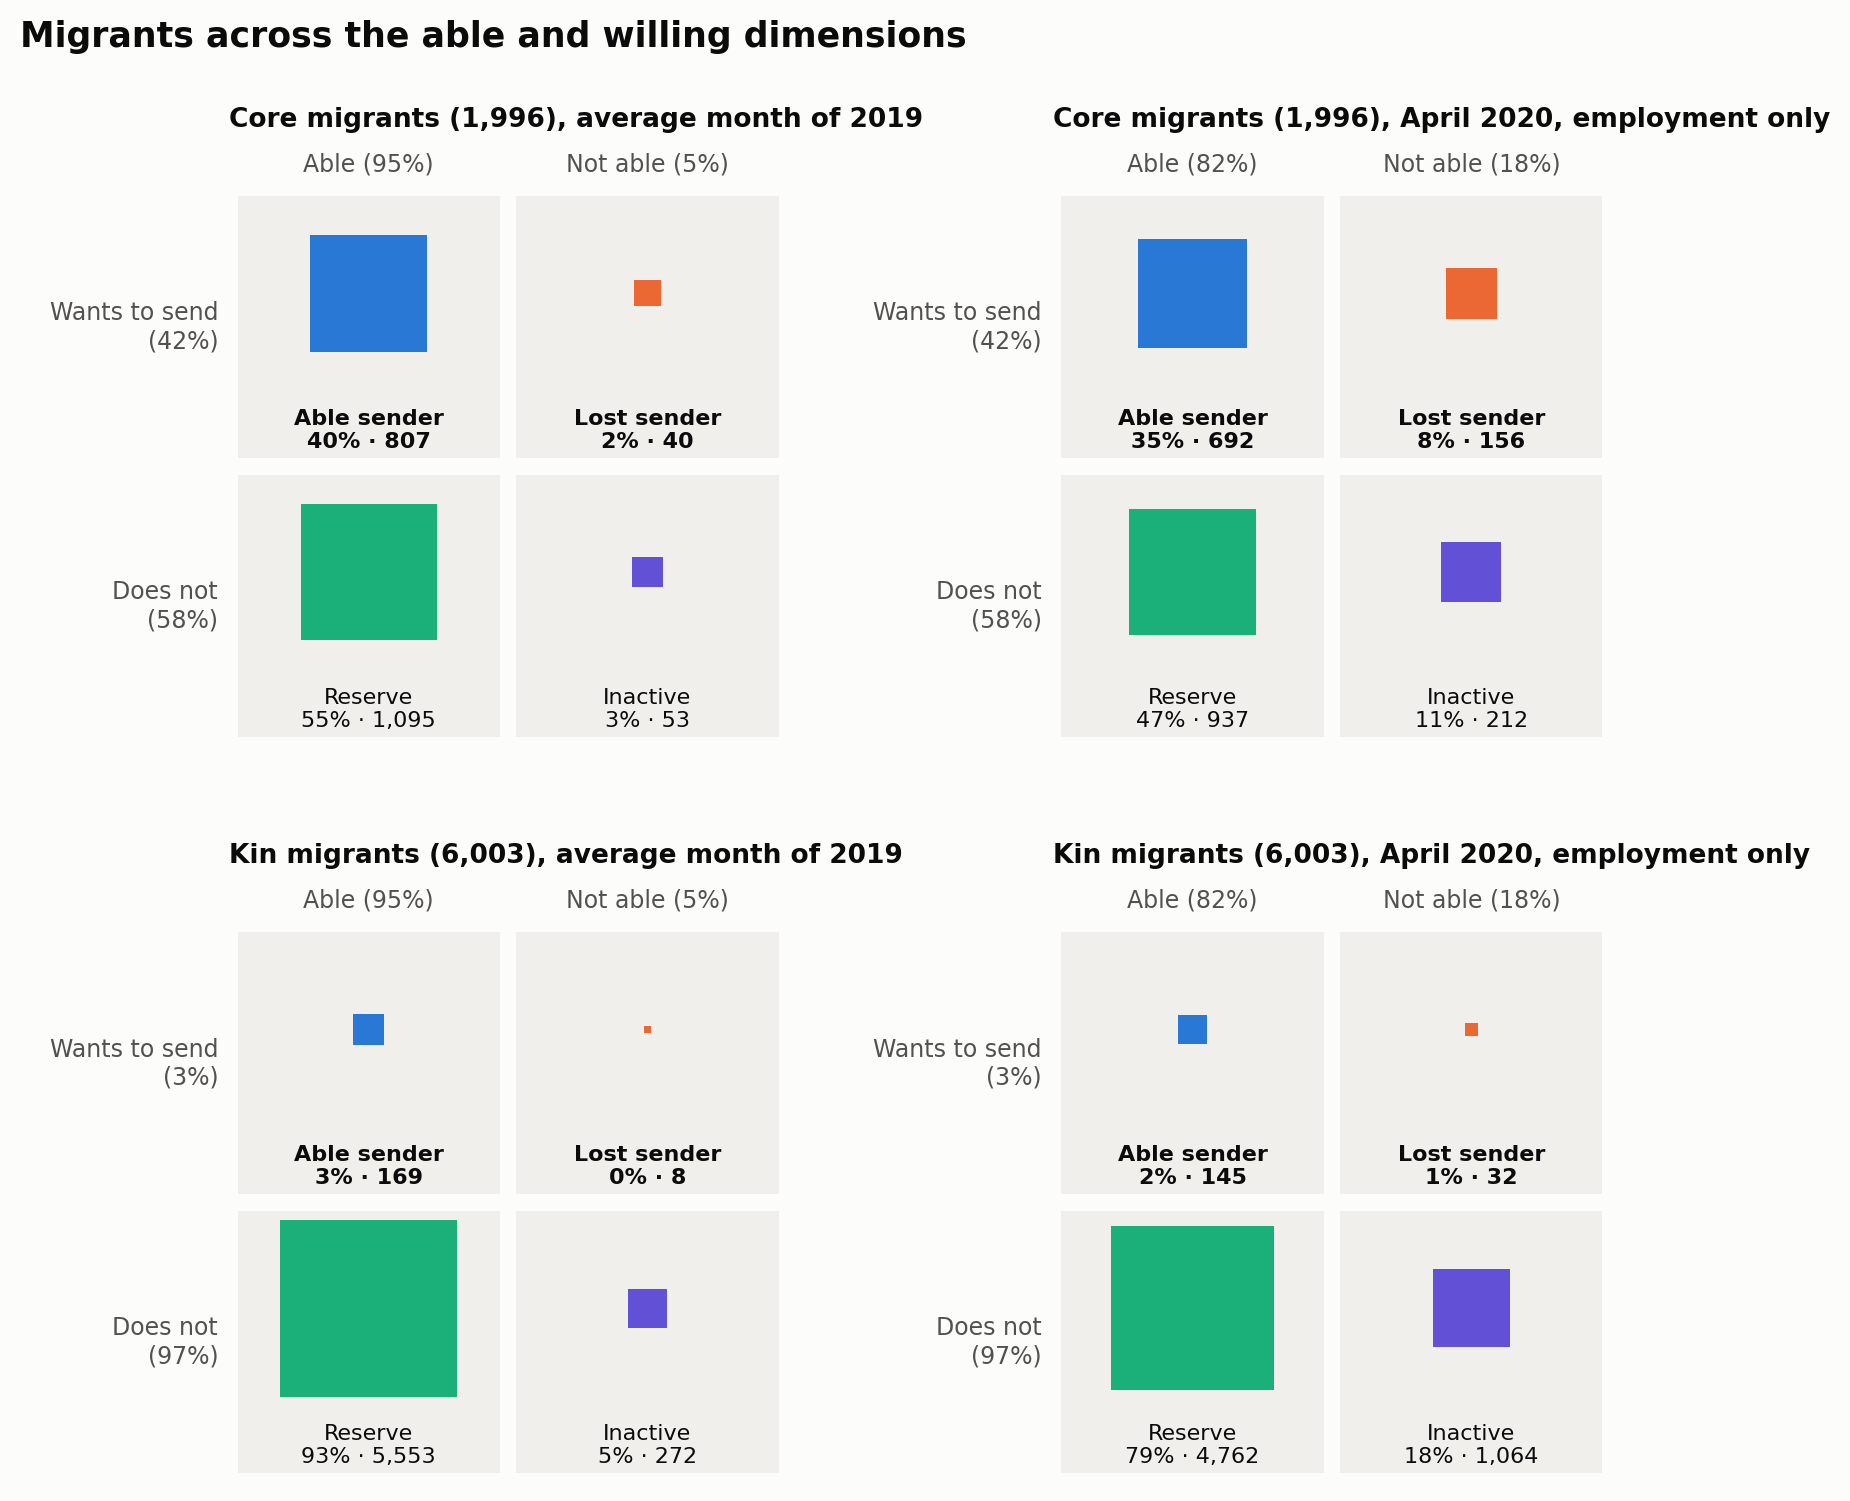
\includegraphics[width=0.9\textwidth]{figures/calibration/C2_able_willing.png}
  \caption{\textbf{Able and willing.} Migrants in each of the four states in a month, for core migrants (top) and kin (bottom), in an average month of 2019 (left) and in April 2020, with that month's employment and 2019 desire (right). Square area is the share of migrants; labels give the share and the number of migrants.}
  \label{fig:able_willing}
\end{figure}

\subsection{When a migrant loses their job}

A lost sender may be replaced by someone in the household's reserve. Each lost sender is replaced with probability $\kappa$, as long as someone in the reserve is available, and the replacement takes over their role:
\begin{equation}
X^c_{h,t} = \min\big(\tilde X^c, R_{h,t}\big), \quad X^k_{h,t} = \min\big(\tilde X^k, R_{h,t} - X^c_{h,t}\big), \qquad \tilde X \sim \mathrm{Binomial}(L_{h,t}, \kappa),
\end{equation}
where $L_{h,t}$ counts lost senders, $R_{h,t}$ the reserve, and core roles are filled first. With $\kappa = 0$ nobody steps in; with $\kappa = 1$ every lost sender is replaced if someone can. A household linked to a single migrant has nobody to step in.

\subsection{From senders to receipt and transfers}

A household receives in a month with a probability that depends on how many able senders it has, counting replacements: $E^c$ core and $E^k$ kin. We use
\begin{equation}
s_h(E^c, E^k) = \expit\Big(b_0 + b_{\mathrm{any}}[E^c > 0] + b_c \log(1 + E^c) + b_{k0}\,[N^c_h = 0]\log(1 + E^k)\Big).
\end{equation}
The first core sender makes the largest difference ($b_{\mathrm{any}}$). Kin count only in households without core migrants ($b_{k0}$). Each able sender sends one transfer in a month in which the household receives, and the national number of transfers is the sum over households. Because migrants' states are independent given the household, the model computes every household's expected receipt and transfers exactly, without simulation.

\subsection{Normal times: calibrating to 2019}

Nine parameters describe normal times and are set from the 2019 survey data, before the pandemic (Table~\ref{tab:params}). We match each household's probability of receiving in an average month of 2019 to its answer in the survey, by maximum likelihood. The survey shows whether a household receives, not who sent, so we proceed in two steps. First, how often each type of migrant wants to send ($a_c$, $a_k$, $g$) comes from how receipt varies with the number of core and kin migrants. Then, with these fixed, we estimate the receipt curve and the need effects. Normal times are calibrated without stepping in, since stepping in is a response to job loss.

\begin{table}[ht]
\centering
\caption{\textbf{Parameters of the model.}}
\label{tab:params}
\begin{tabularx}{\linewidth}{lXrl}
\toprule
Parameter & Meaning & Value & Set from \\
\midrule
$a_c$ & Desire of a household's only core migrant & 0.41 & 2019 survey \\
$a_k$ & Desire of a kin migrant & $-3.40$ & 2019 survey \\
$g$ & Change in core desire with the number of core migrants & $-0.97$ & 2019 survey \\
$\eta_w$, $\eta_o$ & Desire shift: no resident worker; older resident & 0.33, 0.19 & 2019 survey \\
$b_0$, $b_{\mathrm{any}}$, $b_c$, $b_{k0}$ & Receipt curve & $-4.60$, 8.16, 0, 9.70 & 2019 survey \\
\midrule
$\kappa$ & Share of lost senders replaced & 1 & 2020--21 transfers \\
$\beta$ & Response of desire to the crisis in Mexico & 0.15 & 2020--21 transfers \\
$\rho$ & Habit in sending, month to month & 0.93 & ENIGH 2018 \\
\midrule
$\pi$ & Stimulus check lets an out-of-work migrant send & 1 & Assumption \\
\bottomrule
\end{tabularx}
\end{table}

\subsection{Pandemic years: job loss, stepping in and need}

We run the model twice with the same normal-times parameters. The COVID run uses the observed employment of 2020--22, the stimulus checks and the death toll. The no-COVID run uses the employment of the same month of 2019, no checks and no death toll. The model index is the ratio of transfers in the two runs, so, like the data, it measures the pandemic against a world without it. We choose $\kappa$ and $\beta$ to match the data index over the second quarter of 2020 to the end of 2021, and keep 2022 aside as a test. A second check is the size of the jumps in January and March 2021, when stimulus checks arrived: $+4.1$ and $+3.6$ log points above the neighbouring months in the data.

\subsection{Regular sending}

In real families, money tends to come month after month: remittance decisions are persistent, with steady streams more common than one-off bursts \cite{bettin2016steady}, although migrants differ widely in how regularly they engage with home \cite{waldinger2008between}. In ENIGH 2018, half of the households that received money from abroad in the six months before the interview received it in every one of them. We add one habit parameter: a migrant who wanted to send last month is more likely to want to send this month,
\begin{equation}
P(\text{wants}_t \mid \text{wanted}_{t-1}) = d_t - \rho\, d_{t-1} + \rho, \qquad P(\text{wants}_t \mid \text{did not}) = d_t - \rho\, d_{t-1}.
\end{equation}
This form keeps the share of migrants who want to send in each month exactly at $d_t$, so the habit changes \emph{who} sends from month to month but not \emph{how many}: national results are unchanged. We set $\rho = 0.93$ so that the model matches one number, the 2018 share of every-month receivers in ENIGH, and use all other household patterns as tests.

\subsection{Checking the model against other data}

We use three sources the model was not fitted to. ENIGH, Mexico's household income survey \cite{enigh}, records for each household the money received from abroad in each of the six months before the interview, in 2016--22. The 3,749 households of the same communities with no migrant in the United States test the baseline receipt. And the migrant records of the survey say whether household heads sent money during their last US trip.

\subsection{Limits of the data}

The networks are those reported before the pandemic, unweighted and concentrated in the traditional sending regions of western and central Mexico, so they describe this population of migrant families rather than all of Mexico. Kin occupations are imputed. Need at home is measured from household composition, not income. Employment enters as a yes or no condition, without wages or savings. The model counts transfers, not dollars.

%%%%%%%%%%%%%%%%%%%%%%%%%%%%%%%%%%%%%
\section{Results}

\subsection{The model reproduces sending in normal times}

In 2019 a household's only core migrant wants to send in six months out of ten. When a household has two, three or four core migrants, each wants to send less often: in 43\%, 34\% and 28\% of months. Kin want to send in 3\% of months. Without this division of labour, receipt would rise far too steeply with the number of migrants: from 44\% with one core migrant to 93\% with four, against 59\% and 75\% in the survey (Figure~\ref{fig:desire}). With it, the model matches receipt for every family size within two percentage points.

Once a core migrant is an able sender, receipt is close to certain: 97\% in a month. Without any able sender it is 1\%. In households without core migrants, one able kin sender gives 89\%. Need at home raises desire: having no resident worker multiplies a migrant's odds of wanting to send by 1.4, and having an older resident by 1.2.

\begin{figure}[ht]
  \centering
  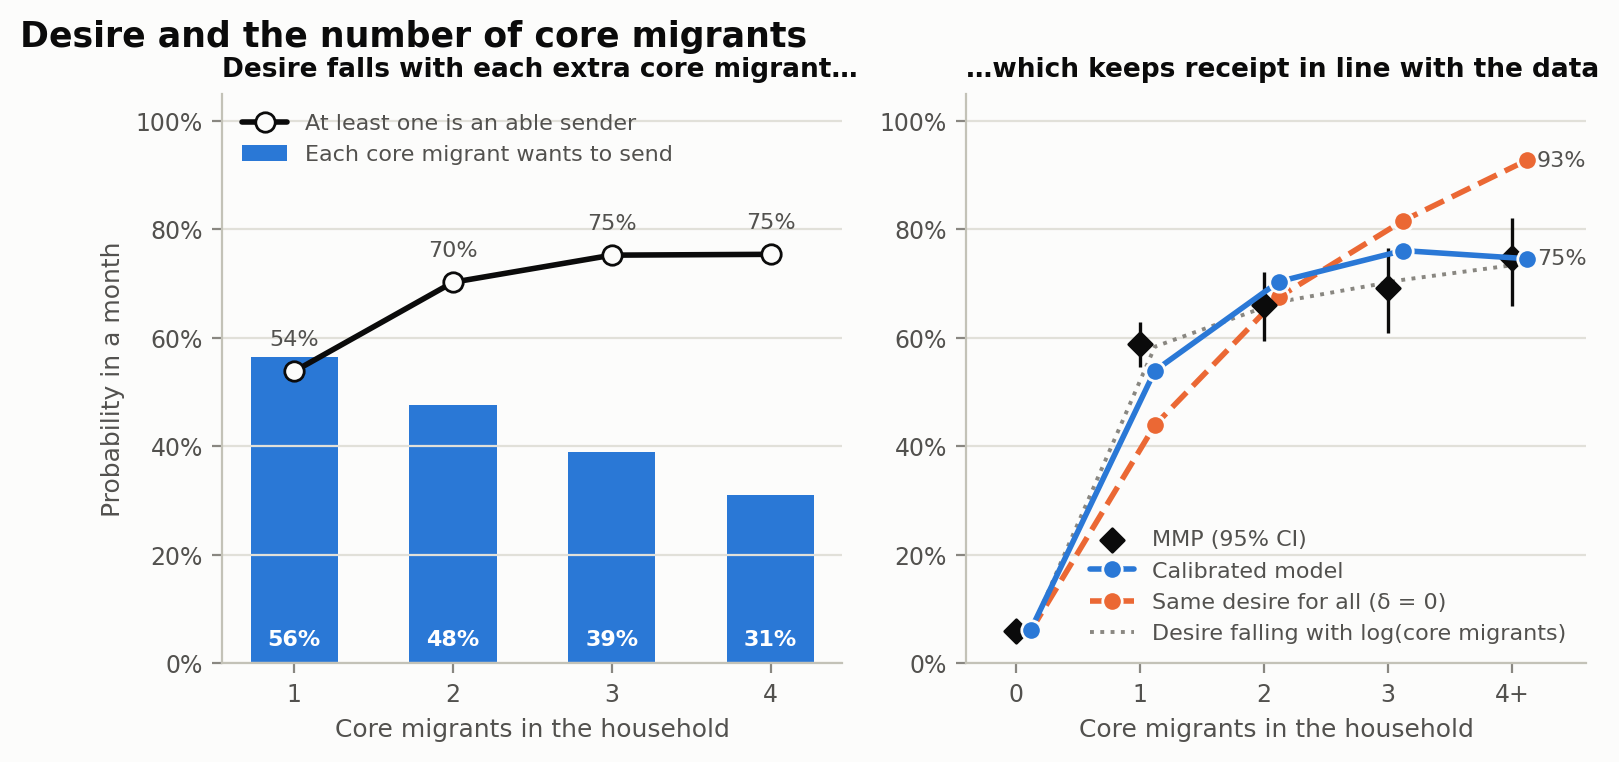
\includegraphics[width=\textwidth]{figures/calibration/C3_desire_network_size.png}
  \caption{\textbf{Desire and the number of core migrants.} (a) Monthly probability that each core migrant wants to send, and that at least one of them is an able sender. (b) Share of households receiving by number of core migrants: survey (95\% intervals), calibrated model, and the model with the same desire for every core migrant ($g = 0$).}
  \label{fig:desire}
\end{figure}

The model separates households into two groups (Figure~\ref{fig:curve}). Households with a core migrant sit high on the receipt curve, between 50\% and 85\% a month. Households linked only to kin sit near the bottom, mostly between 3\% and 25\%. The survey agrees across the whole range. As a check on data not used to fit the model, the 3,730 households of the same communities with no migrant in the United States are predicted to receive in 1.0\% of months; 0.7\% report receiving.

\begin{figure}[ht]
  \centering
  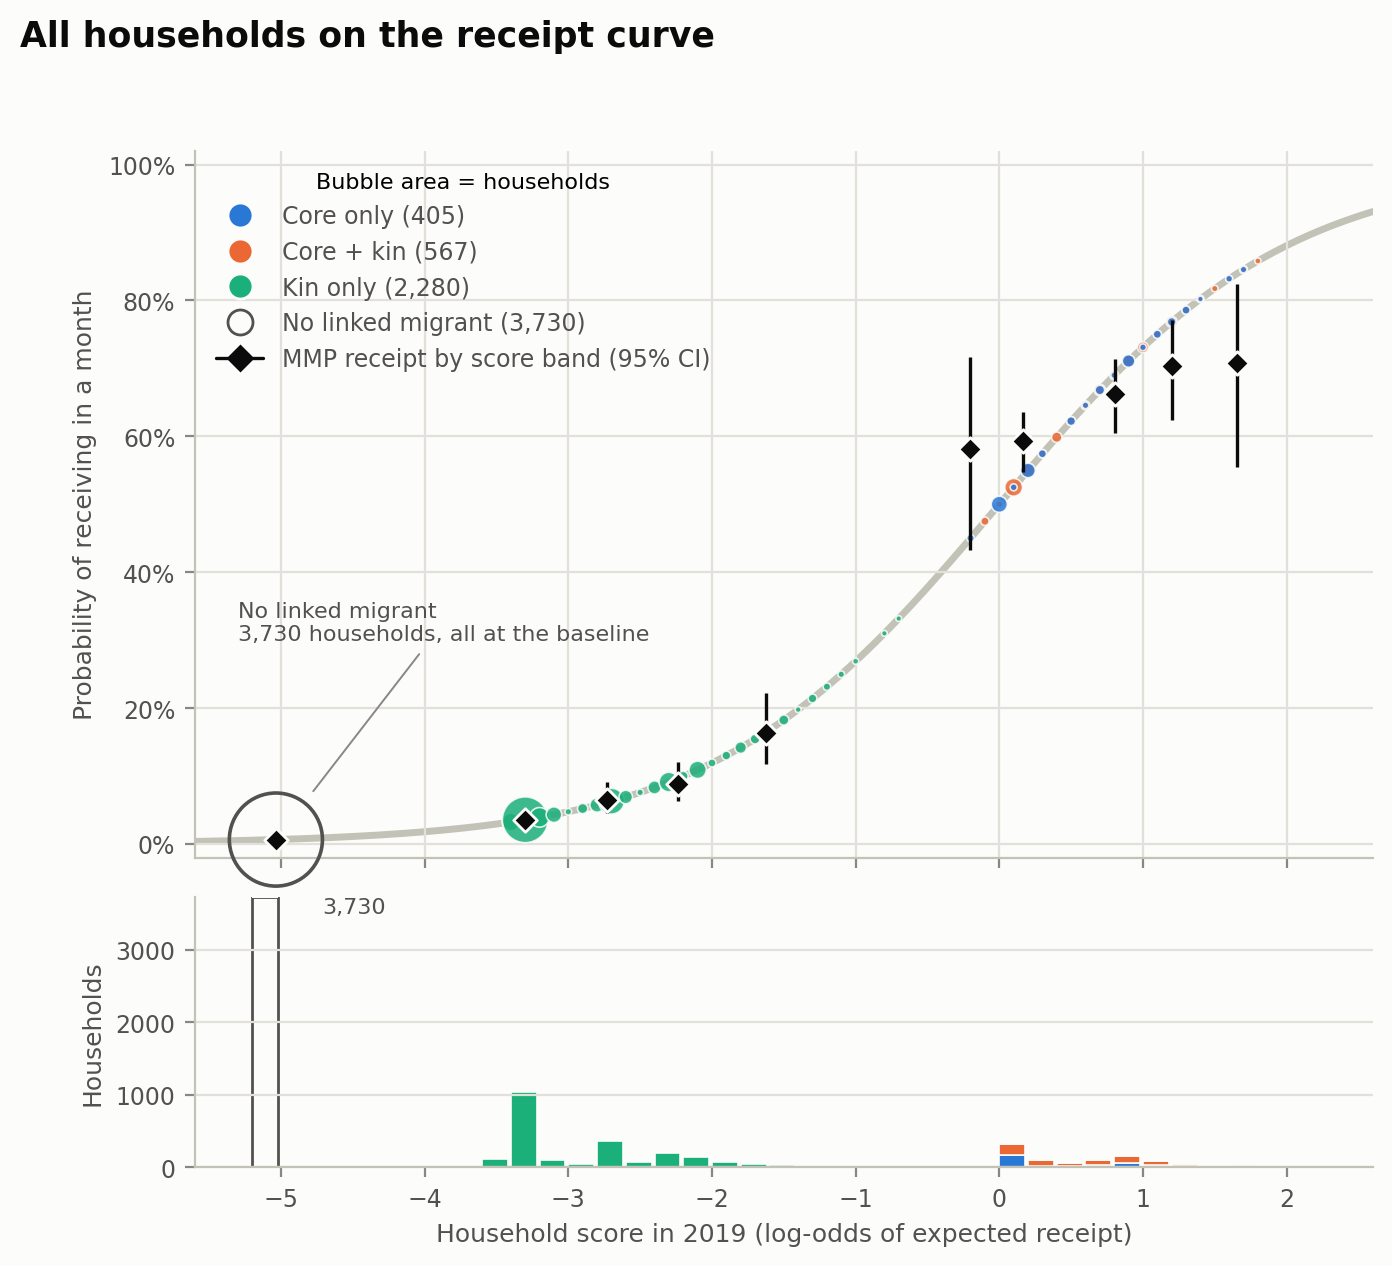
\includegraphics[width=0.8\textwidth]{figures/calibration/C5_households_on_curve.png}
  \caption{\textbf{All households on the receipt curve.} Every household at its expected 2019 receipt, bubbles sized by the number of households. Households with no linked migrant (hollow) are not used to fit the model. Diamonds: receipt reported in the survey, by band (95\% intervals). Bottom: number of households.}
  \label{fig:curve}
\end{figure}

With the habit, the model also reproduces how regularly households receive. In ENIGH 2018, 50\% of receiving households got money in all six months before the interview and 20\% in only one. Without the habit, months are independent and only 5\% receive every month, while 35\% receive once. With the habit set to match the every-month share, 18\% receive once, close to the survey, although too many households receive in five of six months (Figure~\ref{fig:households}a).

\subsection{Families replaced lost senders, and need lifted sending in 2021}

If nothing else had changed, the job losses of spring 2020 would have cut transfers by 12\% in the second quarter, against 3\% in the data (Figure~\ref{fig:national}a, dashed line). Something covered most of the gap. In the model, the gap closes only if relatives stepped in for almost every migrant who lost their job. With full replacement ($\kappa = 1$) the model gives a drop of 2.9\%, against 2.6\% in the data. Without replacement the drop is 11\%, and with half replaced it is 7\%.

\begin{figure}[ht]
  \centering
  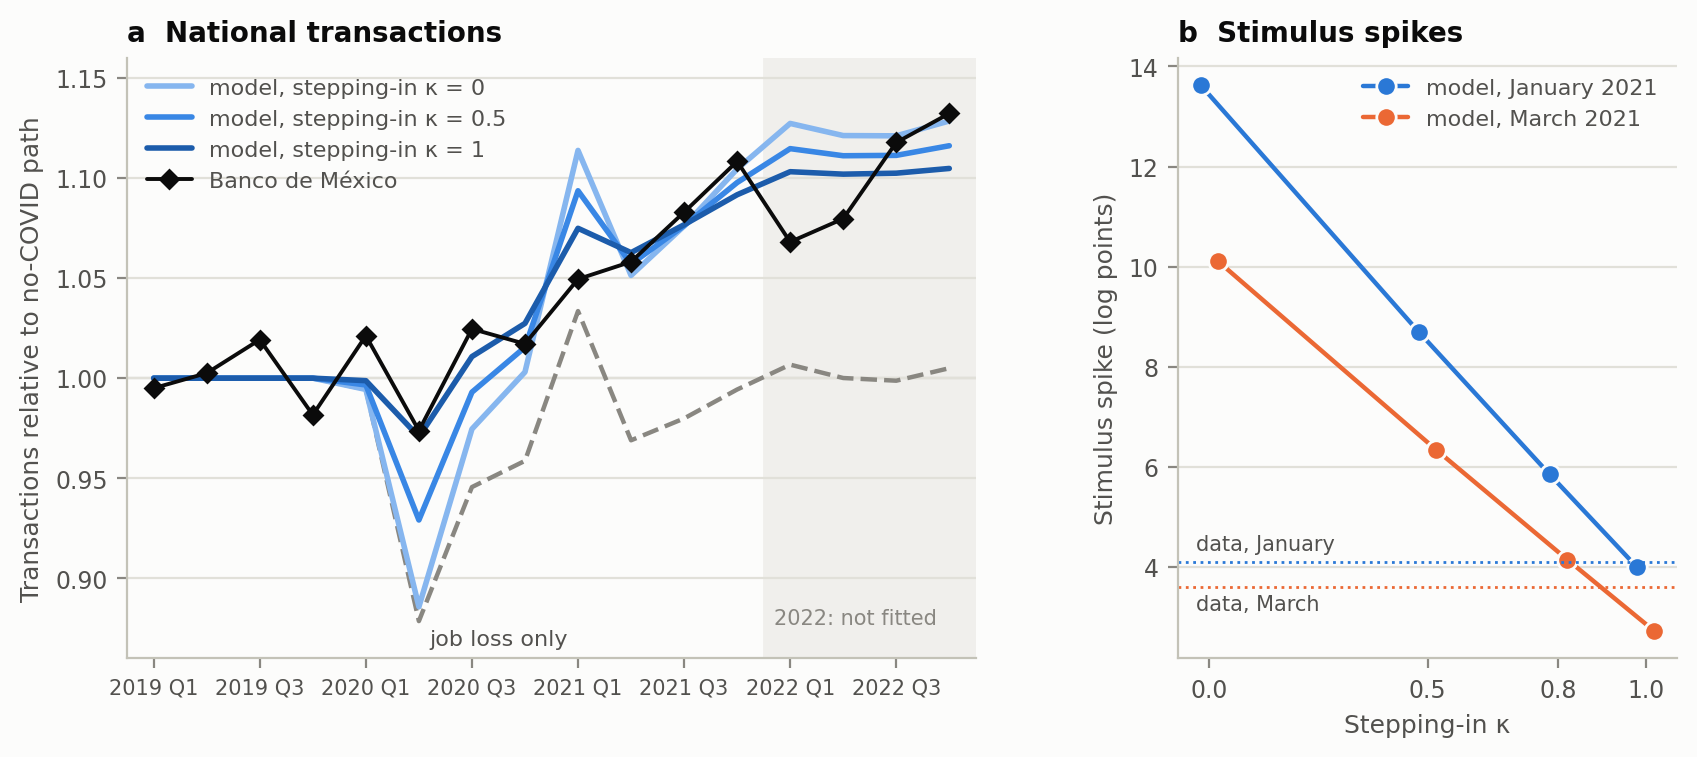
\includegraphics[width=\textwidth]{figures/paper/R1_national_fit.png}
  \caption{\textbf{Job losses, stepping in and need.} (a) Remittance transactions relative to the no-COVID path, quarterly. Dashed: job losses alone. Blue: the model with different shares of lost senders replaced ($\kappa$), each with its best need response. Black: Banco de M\'exico. 2022 (shaded) was not used to fit the model. (b) Size of the jumps in January and March 2021, when stimulus checks arrived, by $\kappa$; dotted lines show the data.}
  \label{fig:national}
\end{figure}

The stimulus checks of 2021 confirm this from a different angle. When a check arrives, migrants who were out of work can send again. If nobody had stepped in for them, the check restores many missing transfers and the monthly number jumps; if relatives had already stepped in, there is little to restore. The data show jumps of 4.1 and 3.6 log points in January and March 2021. Without replacement, the model predicts jumps three times as large; with full replacement it predicts 4.0 and 2.7 (Figure~\ref{fig:national}b). The drop in 2020 and the jumps in 2021 thus bound replacement from both sides: if each lost sender were replaced by more than one relative, the 2020 drop would disappear and the 2021 jumps would turn negative. Replacement was close to one for one.

The rise of 2021 needs a further force. With job losses and replacement alone, transfers return to their trend by 2021. A modest, lasting rise in migrants' wish to send, growing with the cumulative death toll in Mexico, matches the data: a core migrant who wanted to send in 60\% of months in 2019 wants to in 64\% by December 2021. The model then tracks the data from 2020 to 2021 with an average error of 1.3\% per quarter. For 2022, which was not used to fit it, the model predicts 10.3\% above trend; the data show 10.0\%.

How need is measured matters (Figure~\ref{fig:need}). A measure that rises and falls with each wave of deaths sends transfers back to trend as soon as deaths fall, and misses the end of 2021 by ten points. Even a death toll that fades by a tenth each month falls short in 2022. A steady ramp that only marks time since March 2020 fits 2020--21 slightly better but keeps rising and overshoots 2022. The cumulative toll stops rising when deaths stop, and so does the rise in transfers. The national data cannot tell need in Mexico apart from other forces that started in 2020 and lasted, such as savings or new digital channels. But differences across Mexican states and municipalities show no stronger rise where more people died, so the response is to the national crisis, not to local deaths.

\begin{figure}[ht]
  \centering
  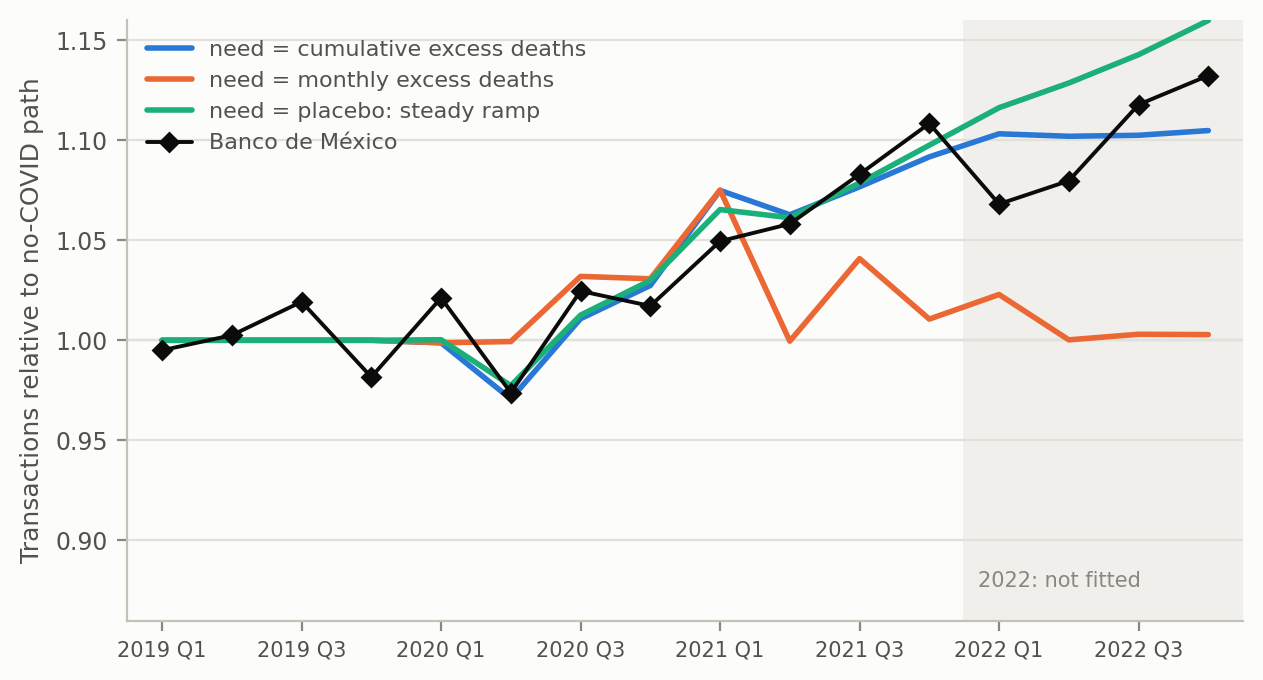
\includegraphics[width=0.75\textwidth]{figures/paper/R2_need_series.png}
  \caption{\textbf{How need is measured.} Remittance transactions relative to the no-COVID path, with full replacement and need measured as the cumulative excess deaths in Mexico, the monthly excess deaths, or a steady ramp since March 2020. Each has its own best response. Black: Banco de M\'exico. 2022 (shaded) was not used to fit the model.}
  \label{fig:need}
\end{figure}

These conclusions hold when we assume migrants want to send more or less often in normal times, under every measure of need, and with or without the habit. One alternative cannot be ruled out with national data: migrants who lost their job might have kept sending at about half their usual rate, from savings or informal work, instead of being replaced. It gives the same national totals. The two stories differ in who loses: under replacement, families with a single migrant; under continued sending, workers in the hardest-hit jobs.

\subsection{Losses fell on few households}

Stepping in protects families with someone to step in. In a household with three children in the United States and two cousins, one child losing their job lowers the chance of receiving in a month from 81\% to 67\%, and a relative stepping in brings it back to 81\% (Figure~\ref{fig:examples}, Supplementary Material). A household whose only migrant is a son who loses his job falls from 57\% to 1\%: nobody can step in. In spring 2020, 29\% of the replacements that would have been needed could not happen, almost all in households like this.

Over April 2020 to December 2021, most households received as often as they would have without the pandemic. The losses fell on few. With regular sending, 2.3\% of households lost at least one month of income from abroad, and 0.6\% lost three or more. Those 0.6\% bore half of all lost months (Figure~\ref{fig:households}b). Without the habit, the same losses would have been spread thinly over more households. Households whose only migrants were close family were hit hardest: 12\% of them lost at least one month, and 3.6\% lost three or more. For these families the loss matters beyond its size: remittance income that becomes irregular is itself a risk that households have to buffer, for example by working more \cite{amuedo2012volatility}.

\begin{figure}[ht]
  \centering
  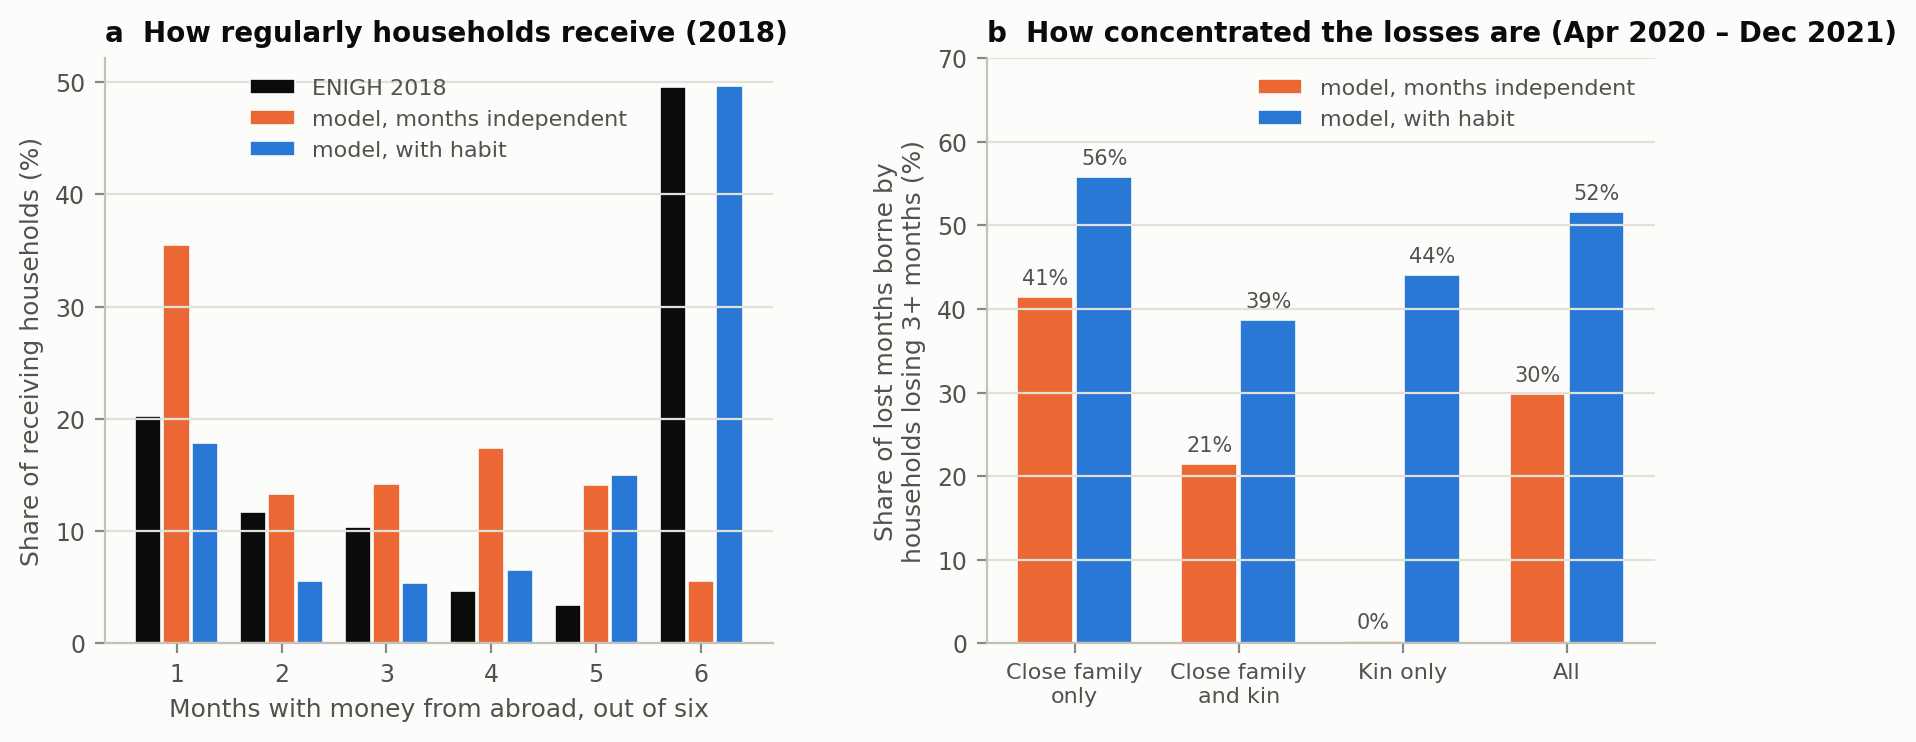
\includegraphics[width=\textwidth]{figures/paper/R3_household_losses.png}
  \caption{\textbf{Who lost out.} (a) Number of months with money from abroad, out of the six before the interview, among receiving households in 2018: ENIGH, the model with independent months, and the model with the habit (set to match the every-month share). (b) Share of all lost months, April 2020 to December 2021, borne by households that lost three or more months, by type of family network.}
  \label{fig:households}
\end{figure}

The household survey supports this picture for 2020. In ENIGH, the share of receiving households that got money every month fell by 2.5 points between 2018 and 2020; the model gives 1.8. The model was not fitted to these changes. It does not reproduce the small fall in the number of households receiving at all (from 4.7\% to 4.4\% of Mexican households), which in the survey goes together with more transfers per receiving household.

By 2022 the survey shows something the model does not explain. The share of Mexican households receiving money from abroad was the same as in 2018, but those households received more regularly: 57\% got money in all six months, up 7.8 points, and the share receiving only once fell by 5.3 points. The model points in the same direction but by much less, 1.4 and 1.2 points. Families did not just receive more; the same families received more steadily. Why remains open.

%%%%%%%%%%%%%%%%%%%%%%%%%%%%%%%%%%%%%
\section{Discussion}

Remittances to Mexico held up during the pandemic because families absorbed the shock. When migrants lost their jobs, relatives in the United States took over their sending, close to one for one, as interviews with migrant families describe \cite{ventura2024resilient}. Our model shows that this is enough to explain why the national totals barely fell in 2020, and that two independent features of the data, the spring drop and the stimulus jumps, both require it.

The rise of 2021 and 2022 is consistent with migrants responding to the scale of the crisis in Mexico as it built up. The response was modest, a few percentage points in how often a migrant wants to send, but lasting, and it predicts 2022 without being fitted to it. This fits the view of remittances as insurance within the family \cite{amuedo2006insurance, sana2005household}, with one twist: the response follows the national toll, not deaths in the migrant's own community.

Stable totals hid concentrated losses. Families linked to a single migrant had nobody to step in. Because sending is a habit, the families that lost money tended to lose it for months, and a small number of them bore half of all lost months. Policies that track remittances only through national totals will miss these households, and support aimed at recipient families in a crisis should look for those that depend on one migrant.

Our results have limits. National data cannot separate stepping in from migrants who kept sending out of savings; the two give the same totals and differ only in who loses. The response to need cannot be told apart, in national data, from other lasting changes that started in 2020, such as the move from informal to formal and digital channels \cite{dinarte2022neither, Bersch2021, amuedo2005use}. The model counts transfers, not dollars: about half of the extra dollars sent in 2021 came from larger transfers, which the model does not explain. The networks come from the traditional sending regions and were recorded before the pandemic.

Two questions remain open. Why did the same families receive more regularly in 2022, when the number of receiving families did not change? And did the families who lost income in 2020 recover it later? Surveys that follow the same households over time, and that record who in the family sends, could answer both.

%%%%%%%%%%%%%%%%%%%%%%%%%%%%%%%%%%%%%%%
\newpage
\printbibliography
% \printbibitembibliography{}

%%%%%%%%%%%%%%

\section*{Acknowledgements}

This work was supported by the Austrian Federal Ministry for Climate Action, Environment, Energy, Mobility, Innovation and Technology (grant number 2021-0.664.668), and by the Asylum, Migration and Integration Fund of the European Commission together with the Federal Ministry of the Interior (grant number 2022-0.392.231).

\section*{Author Contributions}


\section*{Data availability statement}


\section*{Competing Interest Statement}


%%%%%%%%%%%%%%%%%%%%%%%%%

\newpage
\appendix
\section*{Supplementary Material}

\setcounter{figure}{0}
\setcounter{table}{0}

% Redefine numbering to include 'S'
\renewcommand{\thefigure}{S\arabic{figure}}
\renewcommand{\thetable}{S\arabic{table}}

\renewcommand{\thesubsection}{\Alph{subsection}}

\begin{figure}[ht]
  \centering
  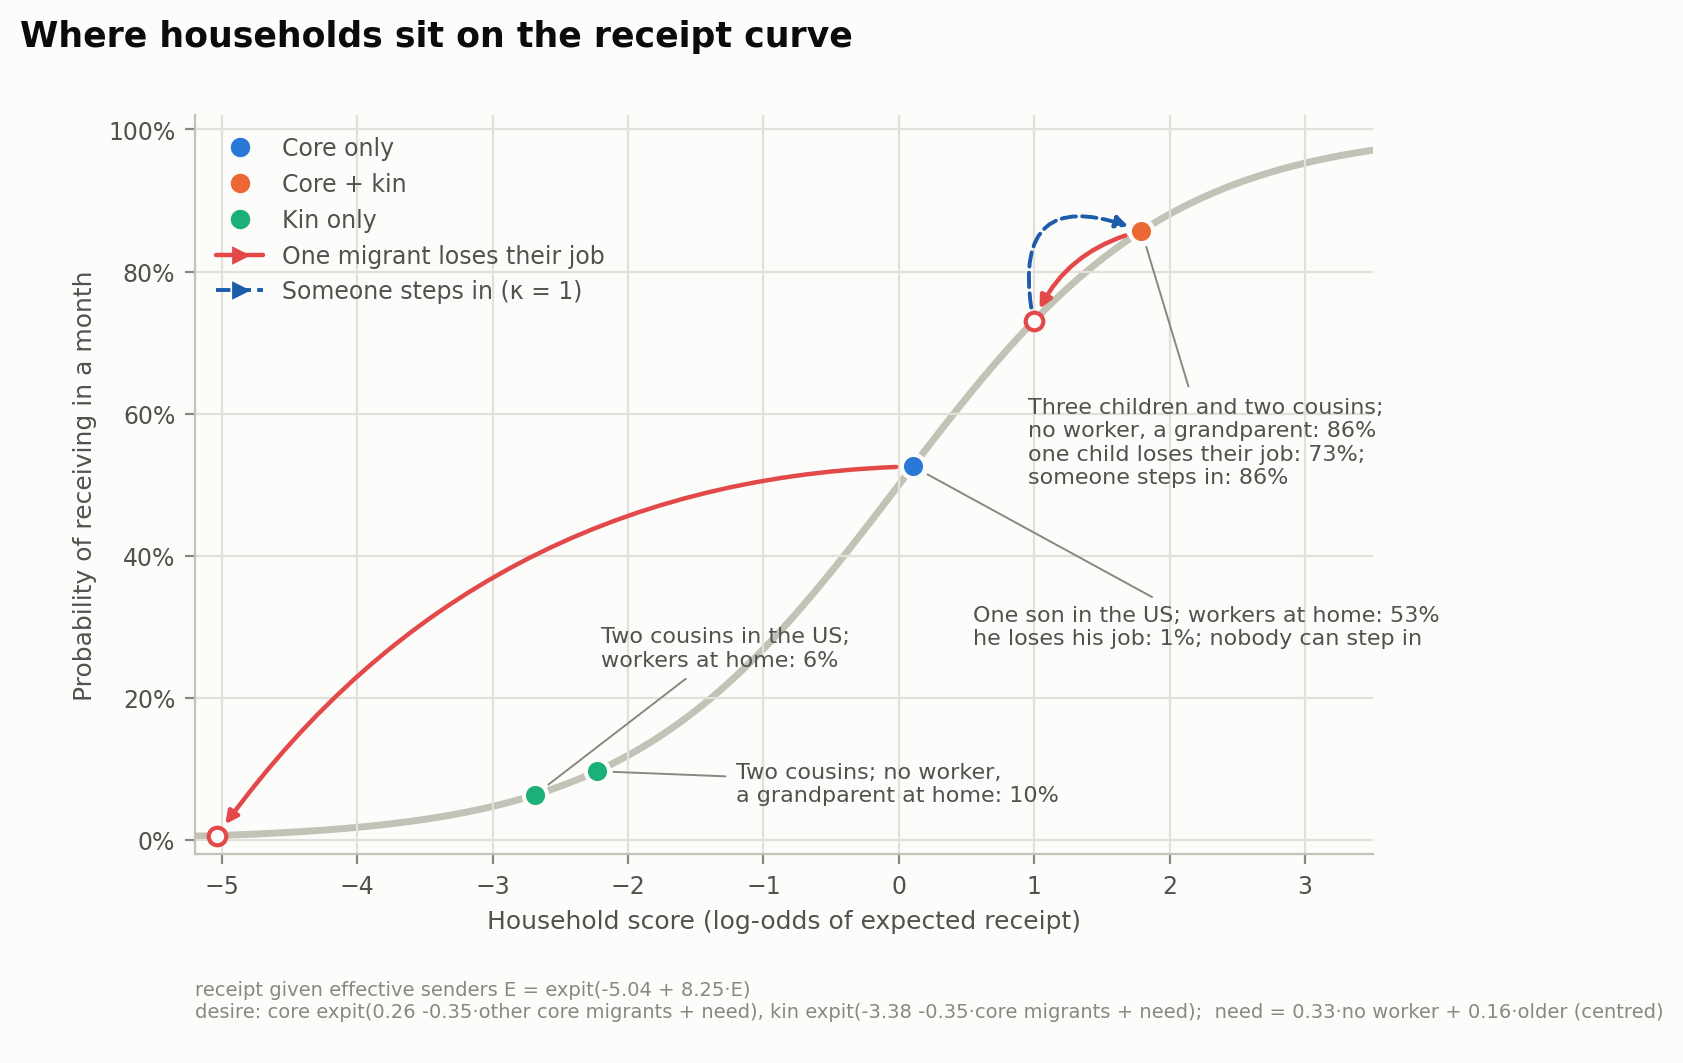
\includegraphics[width=0.8\textwidth]{figures/calibration/C4_receipt_curve_examples.png}
  \caption{\textbf{Where households sit on the receipt curve.} Illustrative families (not survey households), all migrants employed. Red: one migrant loses their job and nobody steps in. Dashed: a relative steps in.}
  \label{fig:examples}
\end{figure}

\begin{figure}[ht]
  \centering
  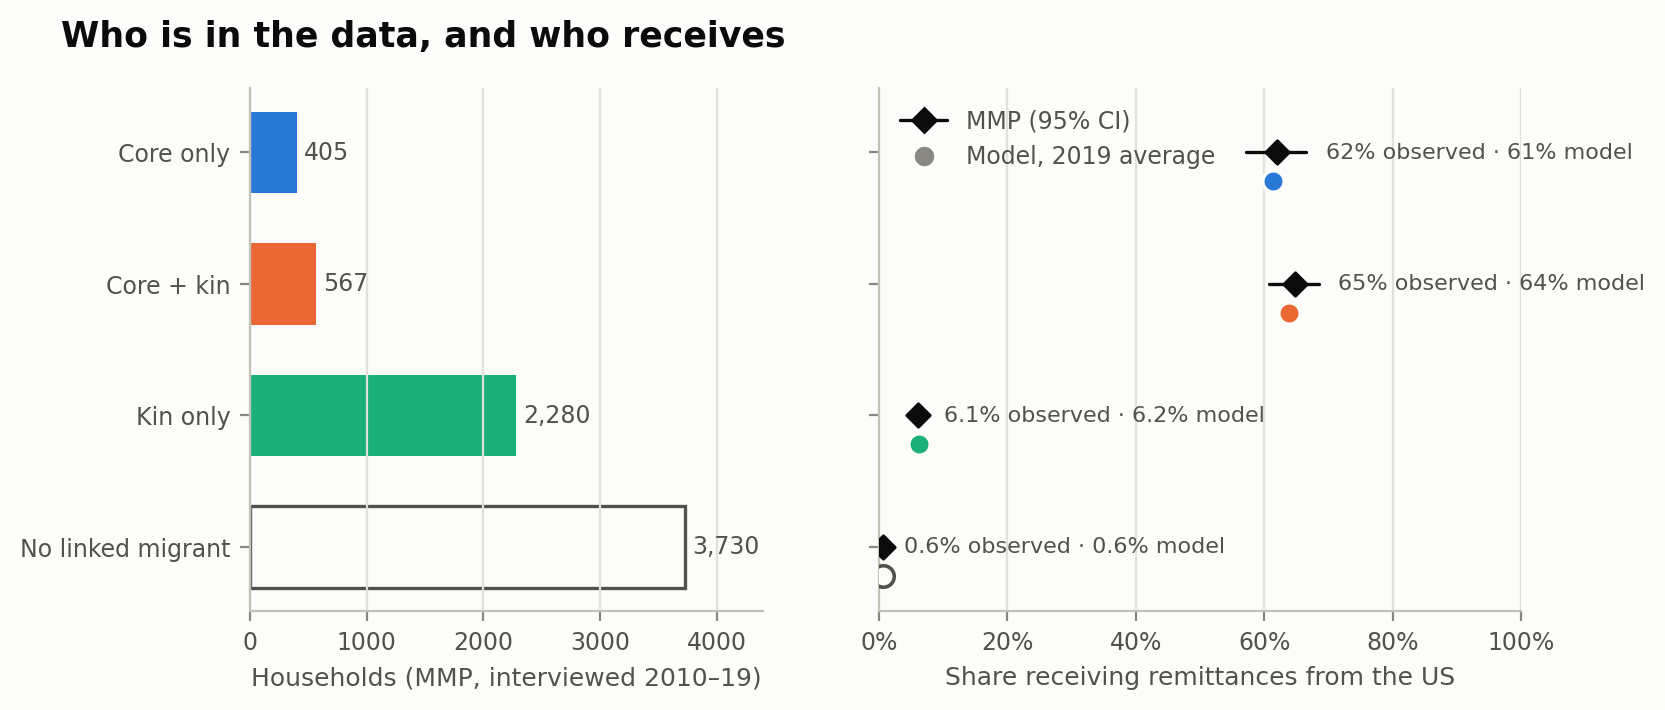
\includegraphics[width=0.9\textwidth]{figures/calibration/C1_households_by_type.png}
  \caption{\textbf{Households in the data.} Households by type of family network, including those with no migrant in the United States, and the share that receives remittances in the survey and in the model.}
  \label{fig:types}
\end{figure}

\begin{figure}[ht]
  \centering
  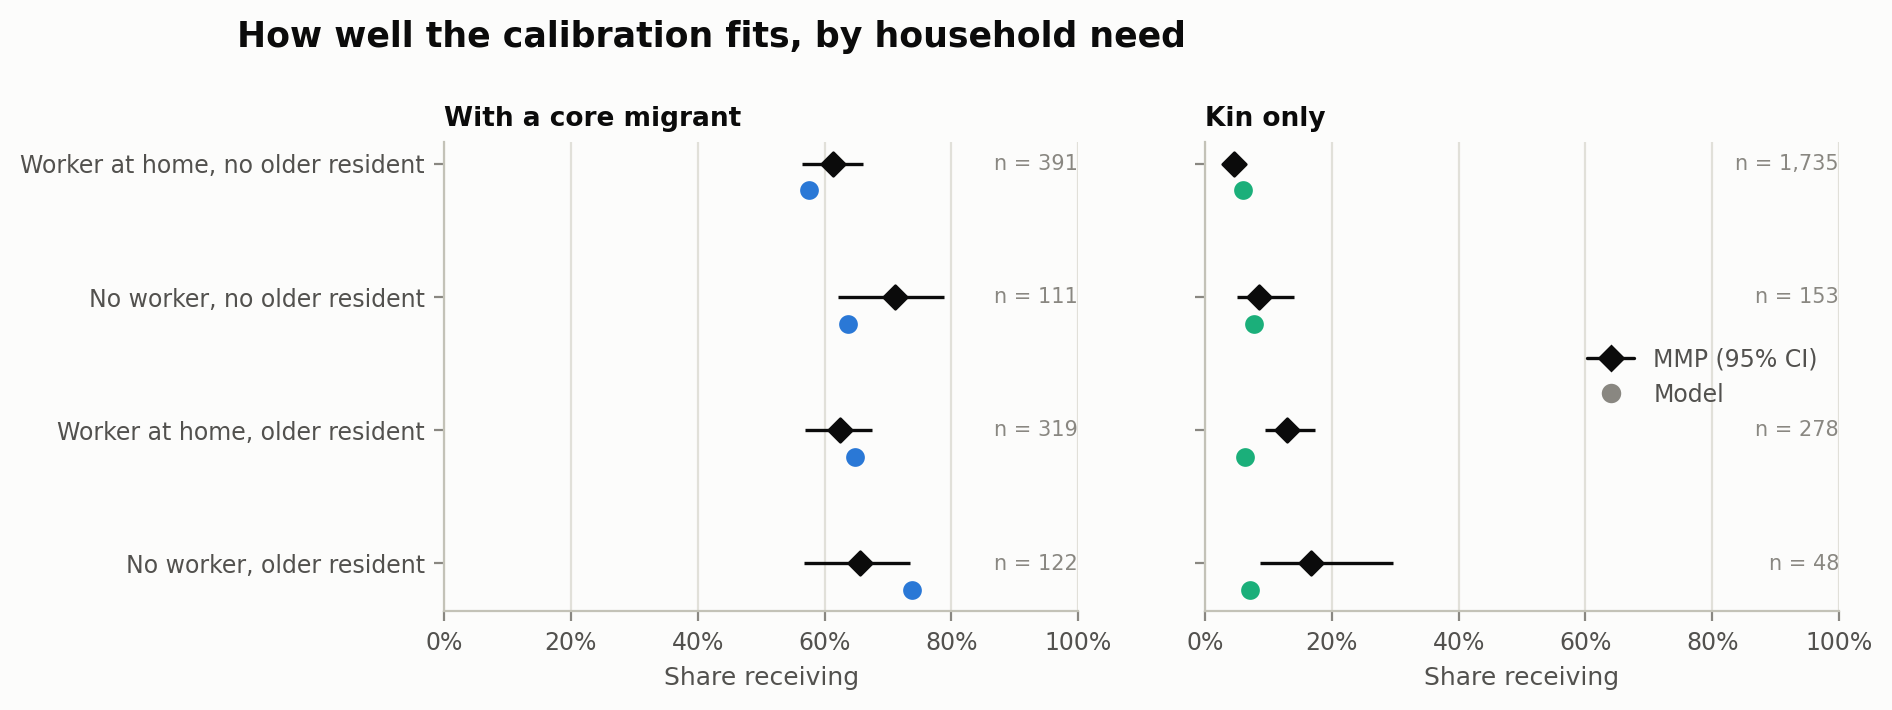
\includegraphics[width=0.9\textwidth]{figures/calibration/C6_fit_by_need.png}
  \caption{\textbf{Fit by household need.} Share of households receiving, survey (95\% intervals) and model, by whether anyone at home works and whether a resident is 65 or older.}
  \label{fig:need_fit}
\end{figure}

\begin{table}[ht]
\centering
\caption{\textbf{Receipt by number of core migrants, survey and model} (2019, 3,252 households).}
\label{tab:fit}
\begin{tabular}{lrccc}
\toprule
Core migrants & Households & Survey & Model & Model, same desire for all \\
\midrule
0 (kin only) & 2,280 & 0.061 & 0.061 & 0.061 \\
1 & 520 & 0.588 & 0.568 & 0.439 \\
2 & 215 & 0.660 & 0.659 & 0.675 \\
3 & 130 & 0.692 & 0.701 & 0.816 \\
4 or more & 107 & 0.748 & 0.758 & 0.927 \\
\bottomrule
\end{tabular}
\end{table}

\end{document}
